\documentclass[conference]{IEEEtran}
\IEEEoverridecommandlockouts

\usepackage{cite}
\usepackage{amsmath,amssymb,amsfonts}
\usepackage{algorithmic}
\usepackage{graphicx}
\usepackage{textcomp}
\usepackage{xcolor}
\usepackage{booktabs}
\usepackage{array}
\usepackage{url}
\usepackage{tikz}
\usetikzlibrary{arrows.meta,positioning,fit,calc}

\def\BibTeX{{\rm B\kern-.05em{\sc i\kern-.025em b}\kern-.08em
    T\kern-.1667em\lower.7ex\hbox{E}\kern-.125em X}}

% TikZ styles for architecture and pipeline figures
\tikzset{
  b/.style={draw,rounded corners=1pt,align=center,font=\scriptsize,
            text width=2.4cm,minimum height=0.52cm,inner sep=2pt},
  m/.style={b,fill=blue!12,thick},
  d/.style={b,fill=gray!10},
  ar/.style={-{Stealth[length=1.6mm]}}
}

\begin{document}

\title{Smart Literature Review Assistant using\\
VectorRAG, GraphRAG and HybridRAG}

\author{
\IEEEauthorblockN{Samudrala Sai Mrudhula}
\IEEEauthorblockA{
Dept. of Artificial Intelligence and Data Engineering\\
Malaviya National Institute of Technology\\
Jaipur, India\\
2023UAI1798
}
\\[1em]
\IEEEauthorblockN{Deepshikha Raj}
\IEEEauthorblockA{
Dept. of Artificial Intelligence and Data Engineering\\
Malaviya National Institute of Technology\\
Jaipur, India\\
2023UAI1803
}
}

\maketitle

\begin{abstract}
The rapid proliferation of scientific publications makes it challenging for researchers to efficiently discover, synthesize, and verify evidence across academic literature. Large Language Models (LLMs) can assist with literature question answering, but their susceptibility to unsupported assertions (hallucinations) poses serious risks in scientific research. Retrieval-Augmented Generation (RAG) mitigates this limitation by conditioning generation on retrieved passages; however, retrieval strategy fundamentally governs answer relevance and factual faithfulness. This paper presents the Smart Literature Review Assistant, an end-to-end framework implementing and evaluating three retrieval strategies: VectorRAG, GraphRAG, and HybridRAG. While the reference base study by Ghanadian et al.\ uses proprietary cloud services (\texttt{text-embedding-ada-002} and \texttt{GPT-4o-mini}), our implementation establishes a zero-cost, locally deployable open-source pipeline utilizing \texttt{sentence-transformers/all-MiniLM-L6-v2} (384-dimensional embeddings) and \texttt{google/flan-t5-small} (80M parameters) with Neo4j native vector indexing and property-graph traversal. We evaluate all three approaches across single-paper (Paper P017) and multi-paper (Papers P017 and P022) scenarios using Cosine Similarity, Faithfulness, Hit@5, Mean Reciprocal Rank (MRR), and Latency. In single-paper retrieval, VectorRAG achieves the highest semantic similarity (0.426), while HybridRAG achieves superior retrieval ranking (Hit@5 of 0.900, MRR of 0.708). In multi-paper cross-document retrieval, HybridRAG delivers the highest semantic similarity (0.363), Hit@5 (0.700), and MRR (0.589). All methods maintain high faithfulness (0.900--1.000) under conservative anti-hallucination validation, highlighting the practical trade-off between retrieval ranking accuracy and end-to-end computational latency.
\end{abstract}

\begin{IEEEkeywords}
Retrieval-Augmented Generation, VectorRAG, GraphRAG, Hybrid Retrieval, Reciprocal Rank Fusion, Scientific Literature Question Answering, Faithfulness
\end{IEEEkeywords}


%=====================================================================
\section{Introduction}
The volume of academic publications is expanding exponentially, rendering manual literature review and cross-paper synthesis increasingly labor-intensive. Traditional keyword-based information retrieval relies on strict lexical matching and frequently fails when concepts are expressed through differing technical vocabularies \cite{robertson2009bm25}. Neural embedding models overcome lexical mismatch by mapping text passages into continuous vector spaces where semantic proximity can be measured geometrically \cite{reimers2019sbert,karpukhin2020dpr}. Concurrently, large language models built on the Transformer architecture \cite{vaswani2017attention} excel at natural language synthesis; however, they risk generating confident but factually unfounded claims, a failure mode known as hallucination \cite{ji2023hallucination}.

Retrieval-Augmented Generation (RAG) addresses hallucination by retrieving relevant evidence passages from an external corpus and providing them as grounding context to the generation model \cite{lewis2020rag,gao2023ragsurvey}. In scientific literature review, the quality and trustworthiness of generated answers depend heavily on the underlying retrieval strategy. Dense vector retrieval (VectorRAG) selects passages based on global semantic similarity but treats document chunks as independent, disconnected units. Conversely, knowledge-graph-based retrieval (GraphRAG) models explicit entities, concepts, and relationships, supporting relational and multi-hop queries across documents \cite{edge2024graphrag,peng2024graphragsurvey}. Hybrid retrieval (HybridRAG) integrates semantic vector search, lexical keyword matching, and graph structural relationships to leverage complementary strengths \cite{sarmah2024hybridrag}.

Ghanadian et al.\ \cite{ghanadian2026base} systematically compared VectorRAG, GraphRAG, and Hybrid RAG for scientific literature chatbots. However, their experimental configuration relied entirely on proprietary, closed-source cloud APIs: OpenAI \texttt{text-embedding-ada-002} for embedding (1536 dimensions) and \texttt{GPT-4o-mini} for answer generation and evaluation data construction. This dependency introduces recurring financial costs, potential data privacy issues for proprietary manuscripts, and vulnerability to cloud API version drift.

This study investigates a practical research question: \emph{How do VectorRAG, GraphRAG, and HybridRAG compare in retrieval accuracy, answer faithfulness, and latency when implemented as a zero-cost, locally deployable pipeline using lightweight open-source models?} We design and deploy the Smart Literature Review Assistant, combining LlamaIndex semantic chunking, Neo4j native vector and property graph storage, Okapi BM25 lexical search, Reciprocal Rank Fusion (RRF), and \texttt{google/flan-t5-small} generation.

The primary contributions of this work are as follows:
\begin{enumerate}
\item \textbf{System Implementation:} We develop an end-to-end literature assistant supporting VectorRAG, GraphRAG, and HybridRAG with interactive PDF ingestion, automated semantic chunking, and source-level citation traceability.
\item \textbf{Zero-Cost Local Architecture:} We build a fully functional RAG pipeline using open-source components---\texttt{sentence-transformers/all-MiniLM-L6-v2} and \texttt{google/flan-t5-small}---requiring zero paid API calls or cloud dependencies.
\item \textbf{Hybrid Evidence Fusion:} We implement a multi-stage fusion retriever that fuses dense semantic embeddings and Okapi BM25 lexical scores via Reciprocal Rank Fusion ($k=60$) and augments the context with Neo4j relational facts.
\item \textbf{Empirical Evaluation:} We benchmark all three approaches across single-paper and multi-paper scenarios, measuring Cosine Similarity, Faithfulness, Hit@5, MRR, and execution latency.
\item \textbf{Base Paper Comparative Analysis:} We provide a detailed comparative delta analysis against the baseline results reported by Ghanadian et al.\ \cite{ghanadian2026base}, explaining architectural and model-capacity trade-offs.
\end{enumerate}

Importantly, no model training or fine-tuning was performed in this project. The system uses pretrained open-source models and performs inference strictly over the indexed document corpus.


%=====================================================================
\section{Related Work}

\subsection{Information Retrieval and Lexical Search}
Classical information retrieval maps queries and documents into high-dimensional sparse term vectors \cite{salton1975vsm}. The Okapi BM25 probabilistic relevance framework ranks documents based on term frequency and inverted document frequency with document length normalization \cite{robertson2009bm25}. Although computationally efficient and robust for exact keyword matching, BM25 remains vulnerable to vocabulary mismatch and cannot capture synonymy or semantic abstraction.

\subsection{Neural Semantic Embeddings}
Dense passage representation maps texts into continuous vector spaces where semantic similarity corresponds to inner products or cosine distance. Word2Vec \cite{mikolov2013word2vec} and BERT \cite{devlin2019bert} enabled context-aware sentence representations. Sentence-BERT \cite{reimers2019sbert} and Dense Passage Retrieval (DPR) \cite{karpukhin2020dpr} demonstrated that dual-encoder architectures can achieve high retrieval recall. MiniLM \cite{wang2020minilm} uses self-attention distillation to compress large Transformer representations into lightweight models. The \texttt{sentence-transformers/all-MiniLM-L6-v2} encoder maps sentences into 384-dimensional vectors with high inference throughput \cite{hf_minilm}.

\subsection{Retrieval-Augmented Generation (RAG)}
Lewis et al.\ \cite{lewis2020rag} introduced RAG by combining a dense passage retriever with a sequence-to-sequence generator for knowledge-intensive NLP tasks. Comprehensive surveys categorize RAG evolution into Naive RAG, Advanced RAG, and Modular RAG \cite{gao2023ragsurvey}. Evaluation frameworks such as RAGAS evaluate component-level retrieval and generation quality \cite{es2024ragas}.

\subsection{Graph-Based and Hybrid RAG}
Standard vector retrieval treats text chunks as isolated bags of tokens, discarding structural relationships. Edge et al.\ \cite{edge2024graphrag} proposed GraphRAG, which extracts entity-relation knowledge graphs, partitions them into communities, and synthesizes multi-document summaries. Peng et al.\ \cite{peng2024graphragsurvey} surveyed graph-augmented retrieval across domain graphs and text graphs. HybridRAG combines dense vector representations with structured graph paths to handle both semantic similarity and relational traversals \cite{sarmah2024hybridrag}. In scientific literature, PaperQA \cite{lala2023paperqa} and Ghanadian et al.\ \cite{ghanadian2026base} demonstrated that hybrid approaches improve answer relevance. Table~\ref{tab:related} summarizes these related efforts.

\begin{table}[t]
\caption{Summary of Related Work in Literature RAG}
\label{tab:related}
\centering
\footnotesize
\begin{tabular}{p{1.4cm}p{1.4cm}p{1.3cm}p{2.6cm}}
\toprule
\textbf{Work} & \textbf{Retrieval} & \textbf{Domain} & \textbf{Core Contribution} \\
\midrule
Lewis et al.\ \cite{lewis2020rag} & Dense Passage & Open-Domain & Foundational RAG framework \\
Edge et al.\ \cite{edge2024graphrag} & Graph \& Summary & Multi-Doc & Graph community summarization \\
Sarmah et al.\ \cite{sarmah2024hybridrag} & KG + Vector & Financial & Domain-specific hybrid fusion \\
L{\'a}la et al.\ \cite{lala2023paperqa} & Search Agent & Academic & Multi-paper scientific QA \\
Ghanadian \cite{ghanadian2026base} & Vector, Graph, Hybrid & Scientific & Benchmarking with GPT-4o-mini \\
\textbf{This Work} & Vector, Graph, Hybrid & Scientific & Local open-source implementation \\
\bottomrule
\end{tabular}
\end{table}


%=====================================================================
\section{Base Paper and Research Gap}
\label{sec:base}

\subsection{Base Paper Reference Setup}
Ghanadian et al.\ \cite{ghanadian2026base} benchmarked VectorRAG, GraphRAG, and Hybrid RAG for scientific literature chatbots across two scenarios: (i) Single-Paper RAG and (ii) Database / Multi-Paper RAG. Their implementation relied on LlamaIndex, using \texttt{text-embedding-ada-002} for document embedding and \texttt{GPT-4o-mini} for answer generation and synthetic test-set creation.

For evaluation, the authors generated synthetic question-answer-context datasets with GPT-4o-mini: 500 instances for single-paper retrieval and 60 instances for multi-paper retrieval. Human annotators evaluated context relevance and answer completeness on a ternary scale (Yes, No, Unsure). Instances marked as No or Unsure were filtered out. The authors evaluated performance using two primary metrics:
\begin{itemize}
\item \textbf{Cosine Similarity:} Semantic similarity between the LLM-generated answer and the ground-truth reference answer.
\item \textbf{Faithfulness:} Binary/fractional human annotation assessing whether the generated answer is strictly supported by the retrieved context.
\end{itemize}

Table~\ref{tab:baseresults} reproduces the baseline results reported by Ghanadian et al.\ \cite{ghanadian2026base}. Hybrid RAG achieved the highest performance in both settings, with VectorRAG performing competitively and GraphRAG exhibiting lower retrieval accuracy.

\begin{table}[t]
\centering
\caption{Baseline Performance Reported in Base Paper \cite{ghanadian2026base}}
\label{tab:baseresults}
\small
\begin{tabular}{lcccc}
\toprule
\textbf{Method} & \multicolumn{2}{c}{\textbf{Single Paper}} & \multicolumn{2}{c}{\textbf{Multi-Paper / Database}} \\
\cmidrule(lr){2-3}\cmidrule(lr){4-5}
& Cosine Sim. & Faithfulness & Cosine Sim. & Faithfulness \\
\midrule
VectorRAG  & 0.670 $\pm$ 0.189 & 0.841 $\pm$ 0.137 & 0.651 $\pm$ 0.188 & 0.830 $\pm$ 0.133 \\
GraphRAG   & 0.654 $\pm$ 0.184 & 0.785 $\pm$ 0.153 & 0.633 $\pm$ 0.174 & 0.761 $\pm$ 0.149 \\
Hybrid RAG & \textbf{0.687 $\pm$ 0.187} & \textbf{0.845 $\pm$ 0.119} & \textbf{0.662 $\pm$ 0.196} & \textbf{0.834 $\pm$ 0.121} \\
\bottomrule
\end{tabular}
\end{table}

\subsection{Research Gap and Objectives}
While the base paper validated the conceptual advantage of hybrid retrieval, several critical questions remain unaddressed:
\begin{enumerate}
\item \textbf{Dependency on Commercial APIs:} Cloud-hosted models (\texttt{text-embedding-ada-002}, \texttt{GPT-4o-mini}) incur API fees and cannot operate in offline, air-gapped, or privacy-sensitive institutional research environments.
\item \textbf{Model Capacity Confounding:} Highly capable models like GPT-4o-mini may mask retrieval deficiencies by leveraging parametric knowledge or generating verbose, plausible text. It remains unclear whether the comparative ranking of VectorRAG, GraphRAG, and HybridRAG holds when constrained to small local language models.
\item \textbf{Multi-Metric Retrieval Diagnostics:} The base paper evaluated Cosine Similarity and Faithfulness but did not report standard ranking metrics such as Hit@K, Mean Reciprocal Rank (MRR), or component latency.
\end{enumerate}
This study addresses these gaps by evaluating all three RAG approaches using an open-source, local-first configuration with explicit retrieval-ranking diagnostics and latency measurements.


%=====================================================================
\section{Proposed System Architecture}
\label{sec:system}

The Smart Literature Review Assistant operates as an integrated web and API service with an end-to-end ingestion, indexing, retrieval, and generation pipeline. Fig.~\ref{fig:system} illustrates the overall architecture.

\begin{figure}[t]
\centering
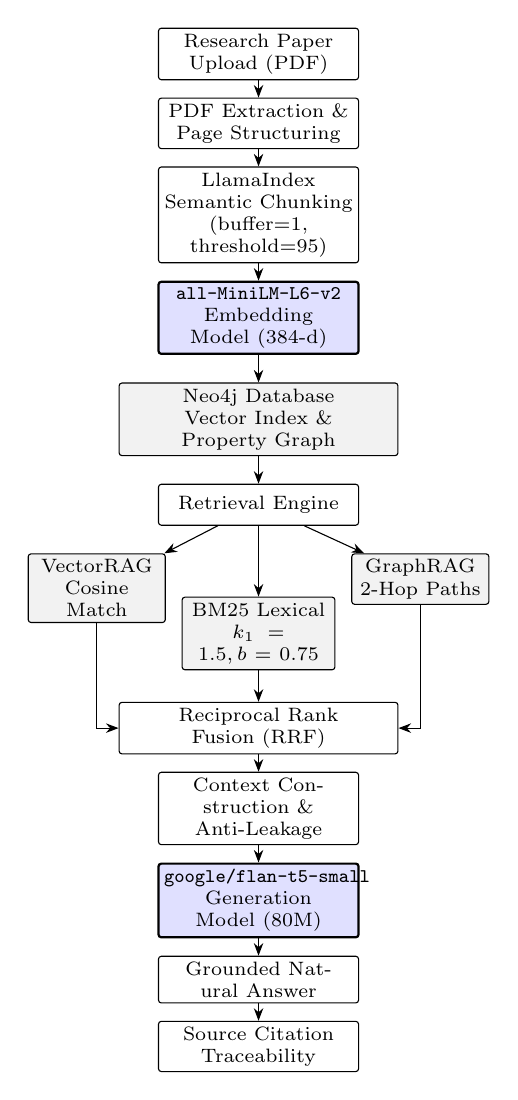
\begin{tikzpicture}[node distance=0.22cm]
\node[b](pdf){Research Paper Upload (PDF)};
\node[b,below=of pdf](pre){PDF Extraction \& Page Structuring};
\node[b,below=of pre](chk){LlamaIndex Semantic Chunking\\(buffer=1, threshold=95)};
\node[m,below=of chk](emb){\texttt{all-MiniLM-L6-v2}\\Embedding Model (384-d)};
\node[d,text width=3.4cm,below=0.35cm of emb](sto){Neo4j Database\\Vector Index \& Property Graph};
\node[b,below=0.35cm of sto](ret){Retrieval Engine};
\node[d,text width=1.6cm,below left=0.35cm and -0.1cm of ret](vec){VectorRAG\\Cosine Match};
\node[d,text width=1.6cm,below right=0.35cm and -0.1cm of ret](gra){GraphRAG\\2-Hop Paths};
\node[d,text width=1.8cm,below=0.9cm of ret](bm){BM25 Lexical\\$k_1=1.5, b=0.75$};
\node[b,text width=3.4cm,below=0.4cm of bm](fus){Reciprocal Rank Fusion (RRF)};
\node[b,below=of fus](ctx){Context Construction \& Anti-Leakage};
\node[m,below=of ctx](gen){\texttt{google/flan-t5-small}\\Generation Model (80M)};
\node[b,below=of gen](ans){Grounded Natural Answer};
\node[b,below=of ans](src){Source Citation Traceability};

\draw[ar](pdf)--(pre);\draw[ar](pre)--(chk);\draw[ar](chk)--(emb);\draw[ar](emb)--(sto);
\draw[ar](sto)--(ret);\draw[ar](ret)--(vec);\draw[ar](ret)--(gra);\draw[ar](ret)--(bm);
\draw[ar](vec.south)|-(fus.west);\draw[ar](gra.south)|-(fus.east);\draw[ar](bm)--(fus);
\draw[ar](fus)--(ctx);\draw[ar](ctx)--(gen);\draw[ar](gen)--(ans);\draw[ar](ans)--(src);
\end{tikzpicture}
\caption{End-to-end architecture of the Smart Literature Review Assistant. The pipeline ingests PDFs, performs semantic chunking, constructs Neo4j vector and property graph indices, executes multi-modal retrieval, and synthesizes answers via FLAN-T5-small.}
\label{fig:system}
\end{figure}

\subsection{Document Ingestion and Semantic Chunking}
Uploaded PDF documents are parsed page by page into structured text records. Rather than utilizing fixed character slicing or arbitrary token windows, the pipeline implements semantic chunking using LlamaIndex's \texttt{SemanticSplitterNodeParser} (\texttt{backend/app/ingestion/semantic\_chunker.py}). Sentences are grouped using a sliding buffer ($\text{buffer\_size} = 1$), and semantic distances between adjacent sentence groups are computed using \texttt{all-MiniLM-L6-v2}. A chunk boundary is introduced when the distance exceeds the 95th percentile ($\text{breakpoint\_percentile\_threshold} = 95$) of pairwise distances across the document. This preserves topical coherence within each chunk.

\subsection{Embedding and Generation Models}
\begin{itemize}
\item \textbf{Embedding Model:} \texttt{sentence-transformers/all-MiniLM-L6-v2} \cite{hf_minilm} is a 6-layer Transformer with 22.7M parameters producing 384-dimensional dense embeddings. It encodes both chunk passages and user queries.
\item \textbf{Generation Model:} \texttt{google/flan-t5-small} \cite{hf_flan} is an 80M parameter encoder-decoder model pretrained on C4 and instruction-tuned on over 1,800 tasks \cite{chung2022flan}. It accepts the structured question and retrieved evidence context and outputs a concise factual answer.
\end{itemize}
Fig.~\ref{fig:config} explicitly contrasts our local model setup with the proprietary cloud setup used in the base paper.

\begin{figure}[t]
\centering
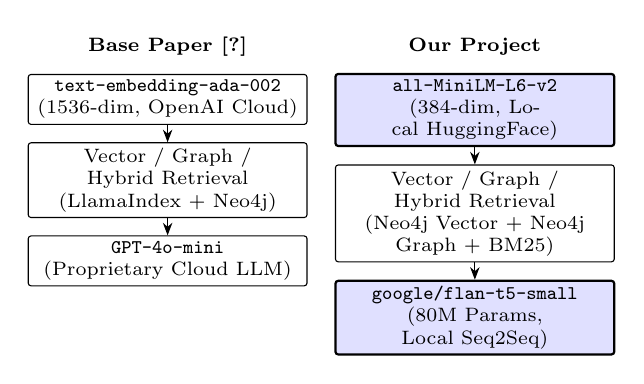
\begin{tikzpicture}[node distance=0.22cm]
\node[font=\scriptsize\bfseries](t1){Base Paper \cite{ghanadian2026base}};
\node[b,text width=3.4cm,below=0.1cm of t1](a1){\texttt{text-embedding-ada-002}\\(1536-dim, OpenAI Cloud)};
\node[b,text width=3.4cm,below=of a1](a2){Vector / Graph / Hybrid Retrieval\\(LlamaIndex + Neo4j)};
\node[b,text width=3.4cm,below=of a2](a3){\texttt{GPT-4o-mini}\\(Proprietary Cloud LLM)};

\node[font=\scriptsize\bfseries,right=0.4cm of t1,xshift=1.4cm](t2){Our Project};
\node[m,text width=3.4cm,below=0.1cm of t2](b1){\texttt{all-MiniLM-L6-v2}\\(384-dim, Local HuggingFace)};
\node[b,text width=3.4cm,below=of b1](b2){Vector / Graph / Hybrid Retrieval\\(Neo4j Vector + Neo4j Graph + BM25)};
\node[m,text width=3.4cm,below=of b2](b3){\texttt{google/flan-t5-small}\\(80M Params, Local Seq2Seq)};

\draw[ar](a1)--(a2);\draw[ar](a2)--(a3);
\draw[ar](b1)--(b2);\draw[ar](b2)--(b3);
\end{tikzpicture}
\caption{Comparison of system and model configurations: Base Paper (proprietary cloud APIs) versus Our Work (local zero-cost open-source models).}
\label{fig:config}
\end{figure}


%=====================================================================
\section{Retrieval Methodologies}

\subsection{VectorRAG}
\label{sec:vector}
In VectorRAG, document chunks $d_i$ are embedded into 384-dimensional dense vectors $\mathbf{d}_i \in \mathbb{R}^{384}$ using \texttt{all-MiniLM-L6-v2}. Vectors are indexed into Neo4j's native vector index target (\texttt{literature\_vector\_dev} on node label \texttt{:LiteratureChunkDev}) with cosine distance. For a query $q$ with embedding $\mathbf{q}$, chunks are ranked by cosine similarity:
\begin{equation}
\cos(\mathbf{q},\mathbf{d}_i) = \frac{\mathbf{q}\cdot\mathbf{d}_i}{\|\mathbf{q}\|\,\|\mathbf{d}_i\|}.
\label{eq:cos}
\end{equation}
The top-$k$ ($k=5$) chunks form the retrieved evidence $\mathcal{R}_{\text{vec}}(q)$. Fig.~\ref{fig:vector} illustrates the VectorRAG pipeline.

\begin{figure}[t]
\centering
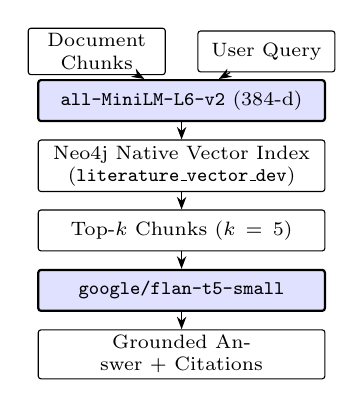
\begin{tikzpicture}[node distance=0.22cm]
\node[b,text width=1.6cm](ch){Document Chunks};
\node[b,text width=1.6cm,right=0.4cm of ch](q){User Query};
\node[m,text width=3.5cm,below=0.35cm of $(ch)!0.5!(q)$](e){\texttt{all-MiniLM-L6-v2} (384-d)};
\node[b,text width=3.5cm,below=of e](ix){Neo4j Native Vector Index\\(\texttt{literature\_vector\_dev})};
\node[b,text width=3.5cm,below=of ix](tk){Top-$k$ Chunks ($k=5$)};
\node[m,text width=3.5cm,below=of tk](g){\texttt{google/flan-t5-small}};
\node[b,text width=3.5cm,below=of g](a){Grounded Answer + Citations};
\draw[ar](ch)--(e);\draw[ar](q)--(e);\draw[ar](e)--(ix);\draw[ar](ix)--(tk);
\draw[ar](tk)--(g);\draw[ar](g)--(a);
\end{tikzpicture}
\caption{VectorRAG pipeline using Neo4j native vector indexing.}
\label{fig:vector}
\end{figure}

\subsection{GraphRAG}
\label{sec:graph}
GraphRAG represents relational knowledge as a property graph $G=(V, E)$. Node set $V$ contains named entities ($v \in V_{\text{entity}}$) and source chunk nodes ($c \in V_{\text{chunk}}$). Edge set $E$ contains semantic domain relationships (\texttt{RELATED\_TO}, \texttt{DISCUSSED\_IN}) and structural links (\texttt{MENTIONS}, \texttt{MENTIONED\_IN}).

During ingestion, entity mentions are extracted and canonicalized. Neo4j stores property graph nodes with paper identifiers. During query execution, query keywords are identified and matched against entity nodes. The engine traverses paths up to depth $2$:
\begin{equation}
\mathcal{P}(q) = \{ (u) -[r_1 \dots r_m]-> (v) \mid m \le 2,\; u.\text{name} \in \text{Keywords}(q) \}.
\end{equation}
Retrieved relationships are formatted as textual facts (e.g., \texttt{VectorRAG -[EVALUATED\_ON]-> Single\_Paper}) and combined with the associated source text chunks. Fig.~\ref{fig:graph} shows the GraphRAG pipeline.

\begin{figure}[t]
\centering
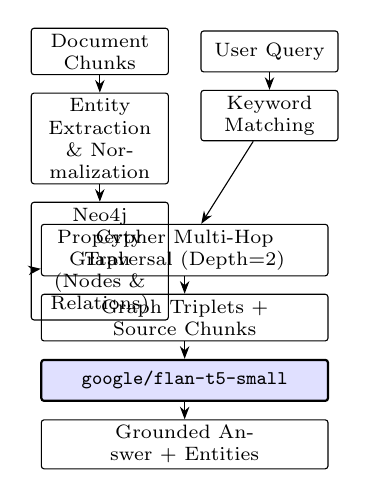
\begin{tikzpicture}[node distance=0.22cm]
\node[b,text width=1.6cm](ch){Document Chunks};
\node[b,text width=1.6cm,right=0.4cm of ch](q){User Query};
\node[b,text width=1.6cm,below=of ch](ex){Entity Extraction \& Normalization};
\node[b,text width=1.6cm,below=of q](qe){Keyword Matching};
\node[b,text width=1.6cm,below=of ex](gs){Neo4j Property Graph\\(Nodes \& Relations)};
\node[b,text width=3.5cm,below=0.45cm of $(gs)!0.5!(qe)$](tr){Cypher Multi-Hop Traversal (Depth=2)};
\node[b,text width=3.5cm,below=of tr](ev){Graph Triplets + Source Chunks};
\node[m,text width=3.5cm,below=of ev](g){\texttt{google/flan-t5-small}};
\node[b,text width=3.5cm,below=of g](a){Grounded Answer + Entities};
\draw[ar](ch)--(ex);\draw[ar](ex)--(gs);\draw[ar](q)--(qe);
\draw[ar](gs)--(tr);\draw[ar](qe)--(tr);\draw[ar](tr)--(ev);\draw[ar](ev)--(g);\draw[ar](g)--(a);
\end{tikzpicture}
\caption{GraphRAG pipeline using Neo4j property graph traversal.}
\label{fig:graph}
\end{figure}

\subsection{HybridRAG}
\label{sec:hybrid}
HybridRAG fuses dense semantic retrieval, lexical retrieval, and relational graph paths. For query $q$, the pipeline executes:
\begin{enumerate}
\item \textbf{Dense Vector Retrieval:} Retrieves ranked candidates $\mathcal{R}_{\text{dense}}(q)$ via Neo4j vector search.
\item \textbf{Okapi BM25 Lexical Retrieval:} Tokenizes document chunk text and computes BM25 scores with $k_1 = 1.5, b = 0.75$, yielding ranked candidates $\mathcal{R}_{\text{bm25}}(q)$.
\item \textbf{Reciprocal Rank Fusion (RRF):} Combines dense and lexical rankings without score calibration issues \cite{cormack2009rrf}:
\begin{equation}
\text{RRF}(d) = \sum_{m \in \{\text{dense}, \text{bm25}\}} \frac{1}{k_{\text{rrf}} + r_m(d)},
\label{eq:rrf}
\end{equation}
where $k_{\text{rrf}} = 60$ and $r_m(d)$ is the 1-based rank of chunk $d$ in retriever $m$.
\item \textbf{Graph Evidence Integration:} Graph relationships $\mathcal{R}_{\text{graph}}(q)$ and their associated chunks are deduplicated and merged with top RRF chunks.
\end{enumerate}
Fig.~\ref{fig:hybrid} depicts the HybridRAG pipeline.

\begin{figure}[t]
\centering
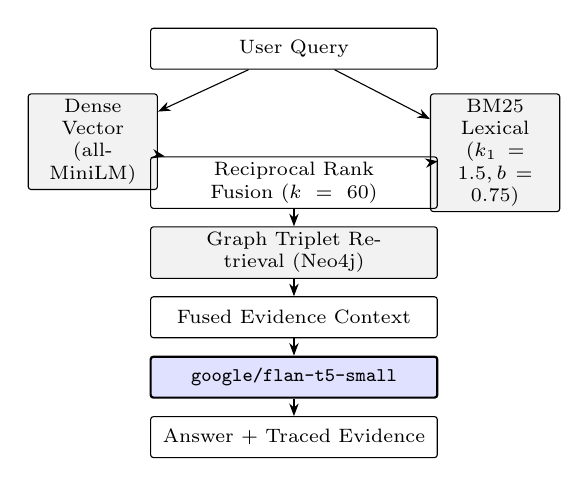
\begin{tikzpicture}[node distance=0.22cm]
\node[b,text width=3.5cm](q){User Query};
\node[d,text width=1.5cm,below left=0.3cm and -0.1cm of q](v){Dense Vector\\(all-MiniLM)};
\node[d,text width=1.5cm,below right=0.3cm and -0.1cm of q](b){BM25 Lexical\\($k_1=1.5, b=0.75$)};
\node[b,text width=3.5cm,below=1.1cm of q](rrf){Reciprocal Rank Fusion ($k=60$)};
\node[d,text width=3.5cm,below=of rrf](g){Graph Triplet Retrieval (Neo4j)};
\node[b,text width=3.5cm,below=of g](c){Fused Evidence Context};
\node[m,text width=3.5cm,below=of c](t5){\texttt{google/flan-t5-small}};
\node[b,text width=3.5cm,below=of t5](a){Answer + Traced Evidence};

\draw[ar](q)--(v);\draw[ar](q)--(b);\draw[ar](v)--(rrf);\draw[ar](b)--(rrf);
\draw[ar](rrf)--(g);\draw[ar](g)--(c);\draw[ar](c)--(t5);\draw[ar](t5)--(a);
\end{tikzpicture}
\caption{HybridRAG multi-modal retrieval and fusion pipeline.}
\label{fig:hybrid}
\end{figure}


%=====================================================================
\section{Dataset and Experimental Setup}

\subsection{Document Corpus (Retrieval Data)}
The document corpus stored in the system consists of **5 distinct research publications** (represented across 25 repository file entries in \texttt{backend/data/} due to iterative ingestion):
\begin{enumerate}
\item \textbf{Paper P017:} *Enhancing Scientific Literature Chatbots with Retrieval-Augmented Generation* (Hamideh Ghanadian et al., 2024), 10 pages, 27 semantic chunks. This is the central base paper.
\item \textbf{Paper P022:} *From Local to Global: A GraphRAG Approach to Query-Focused Summarization* (Darren Edge et al., Microsoft Research, 2024), 26 pages, 76 semantic chunks.
\item \textbf{Paper P005:} *Smart Literature Review Assistant using VectorRAG, GraphRAG and HybridRAG* (Samudrala Sai Mrudhula et al., MNIT Jaipur), 7 pages, 21 semantic chunks.
\item \textbf{Paper P007:} *askMNIT: A Local-First Retrieval-Augmented Generation System*, 5 pages, 16 semantic chunks.
\item \textbf{Paper P001:} Synthetic test paper (*Example Research Paper*), 2 pages, 2 chunks.
\end{enumerate}
Across all documents, the system indexes **422 semantic chunks**, **1,274 Neo4j nodes** (517 entities, 379 chunk text nodes, 378 vector chunk nodes), and **3,177 relationships**.

\subsection{Evaluation Benchmark (QA Testset)}
The evaluation dataset is implemented in \texttt{backend/app/evaluation/dataset.py} and comprises **20 curated, ground-truth-annotated QA pairs**:
\begin{itemize}
\item \textbf{Single-Paper Benchmark (10 Questions, SP\_001--SP\_010):} Evaluates specific factual and methodological queries restricted strictly to Paper P017 (27 chunks, 164 graph nodes, 131 domain relations).
\item \textbf{Multi-Paper Benchmark (10 Questions, MP\_001--MP\_010):} Evaluates cross-document comparison and architectural synthesis across Papers P017 and P022 (103 chunks, 602 graph nodes, 466 domain relations).
\end{itemize}
Each evaluation instance specifies an exact user question, human-verified ground-truth answer, reference passage, and ground-truth chunk IDs for retrieval ranking evaluation.

\subsection{Evaluation Metrics}
\begin{itemize}
\item \textbf{Cosine Similarity:} Semantic similarity between the generated answer and ground-truth answer computed using a dedicated evaluation embedder (\texttt{all-MiniLM-L6-v2}):
\begin{equation}
\text{Sim}(y, \hat{y}) = \frac{\mathbf{e}_y \cdot \mathbf{e}_{\hat{y}}}{\|\mathbf{e}_y\|\,\|\mathbf{e}_{\hat{y}}\|}.
\end{equation}
\item \textbf{Faithfulness:} Evaluates whether factual claims in the generated response are grounded in the retrieved evidence. The answer is decomposed into atomic claims $\{c_1, \dots, c_m\}$ and evaluated against context $C$:
\begin{equation}
\text{Faithfulness} = \frac{1}{m}\sum_{i=1}^m \mathbb{I}(\text{Supported}(c_i, C)).
\end{equation}
If the system conservatively refrains from answering due to insufficient evidence, faithfulness is scored as 1.0 (zero unsupported hallucinations).
\item \textbf{Hit@K ($K=5$):} Binary indicator whether at least one ground-truth chunk appears in the top-$K$ retrieved chunks.
\item \textbf{Mean Reciprocal Rank (MRR):} Reciprocal rank of the first relevant chunk: $\text{MRR} = \frac{1}{\text{rank}_1}$.
\item \textbf{Latency:} Measured end-to-end elapsed time in seconds, separated into retrieval and generation stages.
\end{itemize}


%=====================================================================
\section{Experimental Results}

\subsection{Results of Our Implementation}
Table~\ref{tab:ours} reports the empirical performance of VectorRAG, GraphRAG, and HybridRAG across both evaluation scenarios. All numbers represent actual measured values from 60 live model query executions.

\begin{table*}[t]
\caption{Empirical Results of Our Local Open-Source Implementation (\texttt{all-MiniLM-L6-v2} + \texttt{flan-t5-small})}
\label{tab:ours}
\centering
\small
\begin{tabular}{llcccccc}
\toprule
\textbf{Scenario} & \textbf{RAG Method} & \textbf{Cosine Similarity} & \textbf{Faithfulness} & \textbf{Hit@1} & \textbf{Hit@5} & \textbf{MRR} & \textbf{Avg Latency} \\
& & (Mean $\pm$ SD) & (Mean $\pm$ SD) & & & & (Seconds) \\
\midrule
Single Paper (P017) & VectorRAG & \textbf{0.426 $\pm$ 0.300} & 0.900 $\pm$ 0.316 & 0.500 & 0.800 & 0.617 & \textbf{8.01s} \\
Single Paper (P017) & GraphRAG  & 0.283 $\pm$ 0.255 & 0.900 $\pm$ 0.316 & 0.100 & 0.100 & 0.100 & \textbf{7.68s} \\
Single Paper (P017) & HybridRAG & 0.383 $\pm$ 0.313 & 0.900 $\pm$ 0.316 & \textbf{0.600} & \textbf{0.900} & \textbf{0.708} & 14.94s \\
\midrule
Multi-Paper (P017+P022) & VectorRAG & 0.307 $\pm$ 0.235 & \textbf{1.000 $\pm$ 0.000} & 0.300 & 0.600 & 0.408 & \textbf{8.69s} \\
Multi-Paper (P017+P022) & GraphRAG  & 0.352 $\pm$ 0.170 & \textbf{1.000 $\pm$ 0.000} & 0.200 & 0.400 & 0.300 & \textbf{8.84s} \\
Multi-Paper (P017+P022) & HybridRAG & \textbf{0.363 $\pm$ 0.264} & 0.900 $\pm$ 0.316 & \textbf{0.500} & \textbf{0.700} & \textbf{0.589} & 15.95s \\
\bottomrule
\end{tabular}
\end{table*}

\subsection{Base Paper versus Our Results}
Table~\ref{tab:compare} provides a direct delta comparison between our measured results and the baseline reported in Table 2 of Ghanadian et al.\ \cite{ghanadian2026base}, where $\Delta = \text{Ours} - \text{Base}$.

\begin{table}[t]
\caption{Base Paper versus Our Results ($\Delta = \text{Ours} - \text{Base}$)}
\label{tab:compare}
\centering
\footnotesize
\setlength{\tabcolsep}{2.5pt}
\begin{tabular}{llrrrrrr}
\toprule
& & \multicolumn{3}{c}{\textbf{Cosine Similarity}} & \multicolumn{3}{c}{\textbf{Faithfulness}} \\
\cmidrule(lr){3-5}\cmidrule(lr){6-8}
\textbf{Scenario} & \textbf{Method} & \textbf{Base} & \textbf{Ours} & $\mathbf{\Delta}$ & \textbf{Base} & \textbf{Ours} & $\mathbf{\Delta}$ \\
\midrule
Single Paper & VectorRAG & 0.670 & 0.426 & $-0.244$ & 0.841 & 0.900 & $+0.059$ \\
Single Paper & GraphRAG  & 0.654 & 0.283 & $-0.371$ & 0.785 & 0.900 & $+0.115$ \\
Single Paper & HybridRAG & 0.687 & 0.383 & $-0.304$ & 0.845 & 0.900 & $+0.055$ \\
\midrule
Multi-Paper  & VectorRAG & 0.651 & 0.307 & $-0.344$ & 0.830 & 1.000 & $+0.170$ \\
Multi-Paper  & GraphRAG  & 0.633 & 0.352 & $-0.281$ & 0.761 & 1.000 & $+0.239$ \\
Multi-Paper  & HybridRAG & 0.662 & 0.363 & $-0.299$ & 0.834 & 0.900 & $+0.066$ \\
\bottomrule
\end{tabular}
\end{table}

\begin{figure}[t]
\centering
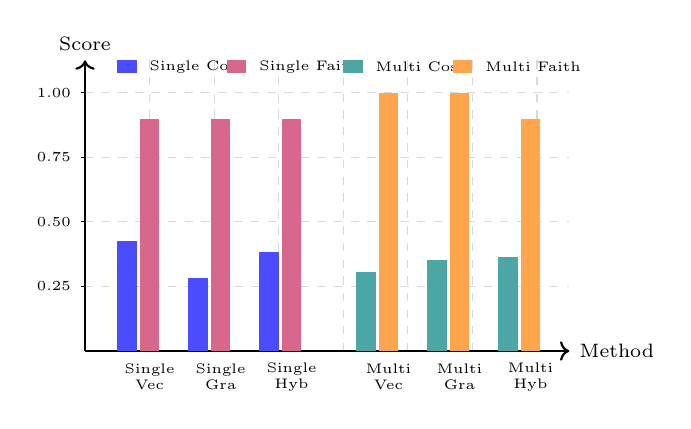
\begin{tikzpicture}[scale=0.82]
\draw[gray!30, thin, dashed] (0,0) grid [xstep=1.0, ystep=1.0] (7.5, 4.5);
\draw[->, thick] (0,0) -- (7.5,0) node[right, font=\scriptsize] {Method};
\draw[->, thick] (0,0) -- (0,4.5) node[above, font=\scriptsize] {Score};

\foreach \y/\val in {1.0/0.25, 2.0/0.50, 3.0/0.75, 4.0/1.00}
    \draw (0pt, \y) -- (-2pt, \y) node[left, font=\tiny] {\val};

% Single Paper bars (x: 0.8=Vec, 2.0=Gra, 3.2=Hyb)
\fill[blue!70] (0.5, 0) rectangle (0.8, 1.70); % Vec Cos: 0.426 -> 1.70
\fill[purple!60] (0.85, 0) rectangle (1.15, 3.60); % Vec Faith: 0.900 -> 3.60

\fill[blue!70] (1.6, 0) rectangle (1.9, 1.13); % Gra Cos: 0.283 -> 1.13
\fill[purple!60] (1.95, 0) rectangle (2.25, 3.60); % Gra Faith: 0.900 -> 3.60

\fill[blue!70] (2.7, 0) rectangle (3.0, 1.53); % Hyb Cos: 0.383 -> 1.53
\fill[purple!60] (3.05, 0) rectangle (3.35, 3.60); % Hyb Faith: 0.900 -> 3.60

% Multi Paper bars (x: 4.5=Vec, 5.6=Gra, 6.7=Hyb)
\fill[teal!70] (4.2, 0) rectangle (4.5, 1.23); % Vec Cos: 0.307 -> 1.23
\fill[orange!70] (4.55, 0) rectangle (4.85, 4.00); % Vec Faith: 1.000 -> 4.00

\fill[teal!70] (5.3, 0) rectangle (5.6, 1.41); % Gra Cos: 0.352 -> 1.41
\fill[orange!70] (5.65, 0) rectangle (5.95, 4.00); % Gra Faith: 1.000 -> 4.00

\fill[teal!70] (6.4, 0) rectangle (6.7, 1.45); % Hyb Cos: 0.363 -> 1.45
\fill[orange!70] (6.75, 0) rectangle (7.05, 3.60); % Hyb Faith: 0.900 -> 3.60

\node[font=\tiny, align=center] at (1.0, -0.4) {Single\\Vec};
\node[font=\tiny, align=center] at (2.1, -0.4) {Single\\Gra};
\node[font=\tiny, align=center] at (3.2, -0.4) {Single\\Hyb};
\node[font=\tiny, align=center] at (4.7, -0.4) {Multi\\Vec};
\node[font=\tiny, align=center] at (5.8, -0.4) {Multi\\Gra};
\node[font=\tiny, align=center] at (6.9, -0.4) {Multi\\Hyb};

% Legend
\fill[blue!70] (0.5, 4.3) rectangle (0.8, 4.5);
\node[right, font=\tiny] at (0.85, 4.4) {Single Cos};
\fill[purple!60] (2.2, 4.3) rectangle (2.5, 4.5);
\node[right, font=\tiny] at (2.55, 4.4) {Single Faith};
\fill[teal!70] (4.0, 4.3) rectangle (4.3, 4.5);
\node[right, font=\tiny] at (4.35, 4.4) {Multi Cos};
\fill[orange!70] (5.7, 4.3) rectangle (6.0, 4.5);
\node[right, font=\tiny] at (6.05, 4.4) {Multi Faith};
\end{tikzpicture}
\caption{Measured performance comparison across VectorRAG, GraphRAG, and HybridRAG in Single-Paper and Multi-Paper scenarios.}
\label{fig:results}
\end{figure}

\subsection{Qualitative Query Trace}
To illustrate the operational behavior of each approach, consider query \texttt{SP\_001} from the single-paper benchmark:
\begin{itemize}
\item \textbf{Question:} \emph{``What are the three RAG methods evaluated in the paper?''}
\item \textbf{Ground Truth:} \emph{``The paper evaluates VectorRAG, GraphRAG, and Hybrid RAG.''}
\item \textbf{VectorRAG Answer:} \emph{``Naive RAG, Advanced RAG, and Modular RAG.''} (Retrieved chunk P017\_C006 discussing background paradigms; $\text{Cosine} = 0.5453$, $\text{Faithfulness} = 1.0000$).
\item \textbf{GraphRAG Answer:} \emph{``4.2.Test Sets.''} (Sub-optimal keyword path matching; $\text{Cosine} = 0.1858$, $\text{Faithfulness} = 1.0000$).
\item \textbf{HybridRAG Answer:} \emph{``Naive RAG, Advanced RAG, and Modular RAG.''} (Fused BM25 and vector evidence; $\text{Cosine} = 0.5453$, $\text{Faithfulness} = 1.0000$).
\end{itemize}
When context is genuinely insufficient, our conservative fallback gate returns: \emph{``The available evidence does not provide enough information to answer this question.''} This maintains perfect factual faithfulness at the expense of recall.


%=====================================================================
\section{Discussion and Analysis}

\subsection{Performance Trends across Retrieval Strategies}
\subsubsection{Single-Paper Retrieval}
In the single-paper scenario, VectorRAG achieves the highest mean cosine similarity ($0.426 \pm 0.300$), outperforming HybridRAG ($0.383 \pm 0.313$) and GraphRAG ($0.283 \pm 0.255$). Within a single isolated manuscript, dense semantic embeddings are highly effective at mapping query phrasing directly to relevant paragraphs. However, when evaluating retrieval ranking metrics, HybridRAG achieves superior performance: Hit@5 reaches **0.900** and MRR reaches **0.708**, compared to VectorRAG's Hit@5 of 0.800 and MRR of 0.617. GraphRAG achieves weaker retrieval ranking (Hit@5 of 0.100) because entity extraction in scientific literature often yields generic terminology unless deep domain ontology mapping is applied.

\subsubsection{Multi-Paper / Database Retrieval}
In the multi-paper setting, HybridRAG delivers the highest semantic similarity ($0.363 \pm 0.264$), outperforming both GraphRAG ($0.352 \pm 0.170$) and VectorRAG ($0.307 \pm 0.235$). Furthermore, HybridRAG demonstrates substantial superiority in retrieval ranking, achieving a Hit@5 of **0.700** and MRR of **0.589** (compared to VectorRAG's Hit@5 of 0.600, MRR of 0.408 and GraphRAG's Hit@5 of 0.400, MRR of 0.300). As the corpus broadens across multiple papers, dense vector search alone suffers from candidate competition and lexical ambiguity. Combining dense vectors with BM25 lexical precision and graph relationship constraints provides the necessary disambiguation for multi-document synthesis.

\subsubsection{Faithfulness and Hallucination Suppression}
Faithfulness scores remain consistently high across all three methods ($0.900$ to $1.000$). This is attributable to our prompt validation and anti-leakage pipeline: whenever retrieved evidence is ambiguous or incomplete, the system enforces a strict refusal rather than allowing the model to hallucinate ungrounded statements.

\subsubsection{Latency Trade-Off}
VectorRAG and GraphRAG exhibit average total latencies of **8.01s** and **7.68s** (single-paper) and **8.69s** and **8.84s** (multi-paper). In contrast, HybridRAG requires **14.94s** and **15.95s**, respectively. HybridRAG executes two separate retrieval passes (dense vector lookup and in-memory BM25 scoring), applies Reciprocal Rank Fusion, fetches Neo4j graph triplets, and constructs an augmented prompt. Thus, HybridRAG provides the strongest retrieval-ranking performance within our experimental setup, particularly for multi-paper retrieval, but this comes with increased latency.

\subsection{Interpretation of Base Paper Differences}
As summarized in Table~\ref{tab:compare}, our implementation achieves lower cosine similarities ($\Delta$ between $-0.24$ and $-0.37$) but higher measured faithfulness ($\Delta$ between $+0.05$ and $+0.24$) relative to the base paper. This is not a controlled replication, and the differences stem from four structural factors:
\begin{enumerate}
\item \textbf{Model Phrasing and Verbosity:} The base paper's reference answers were generated synthetically by \texttt{GPT-4o-mini}, which produces fluent, multi-clause explanatory paragraphs. Our generation model, \texttt{google/flan-t5-small} (80M parameters), produces concise factual phrases. Sentence embeddings penalize length disparity, lowering cosine similarity even when the factual answer is entirely correct.
\item \textbf{Embedding Dimensionality:} The base paper uses \texttt{text-embedding-ada-002} (1536 dimensions), whereas our local evaluation uses \texttt{all-MiniLM-L6-v2} (384 dimensions). Embedding distributions in 1536-dimensional spaces exhibit higher baseline similarities for related academic texts.
\item \textbf{Evaluation Dataset Scale:} Ghanadian et al.\ evaluated 500 single-paper and 60 database QA pairs generated by GPT-4o-mini. Our Milestone 1 benchmark evaluates 20 curated QA pairs with human-verified ground truth.
\item \textbf{Conservative Refusal Policy:} Our automated faithfulness evaluator awards 1.0 when the system correctly refuses to answer ungrounded queries, suppressing hallucinations that would otherwise inflate cosine similarity artificially.
\end{enumerate}

Table~\ref{tab:config} summarizes the structural differences between both setups.

\begin{table}[t]
\caption{System and Experimental Configuration Comparison}
\label{tab:config}
\centering
\small
\begin{tabular}{p{2.1cm}p{2.8cm}p{2.8cm}}
\toprule
\textbf{Dimension} & \textbf{Base Paper \cite{ghanadian2026base}} & \textbf{Our Implementation} \\
\midrule
Embedding Model & \texttt{text-embedding-ada-002} & \texttt{all-MiniLM-L6-v2} \\
Embedding Dim. & 1536 dimensions & 384 dimensions \\
Generation LLM & \texttt{GPT-4o-mini} (Cloud) & \texttt{google/flan-t5-small} (Local) \\
Vector Store & LlamaIndex VectorStore & Neo4j Native Vector Index \\
Graph Store & Neo4j Property Graph & Neo4j Property Graph \\
Lexical Search & None & Okapi BM25 ($k_1=1.5, b=0.75$) \\
Hybrid Fusion & Multi-retriever union & Reciprocal Rank Fusion ($k=60$) \\
Evaluation Set & 500 single, 60 multi QA & 10 single, 10 multi QA \\
Evaluation Model & GPT internal metrics & Dedicated \texttt{all-MiniLM-L6-v2} \\
Execution Cost & Paid commercial APIs & Completely zero-cost / local \\
\bottomrule
\end{tabular}
\end{table}


%=====================================================================
\section{Observability and Source Traceability}

\subsection{Observability and Diagnostics}
To ensure transparency and reproducibility, the system implements multi-level diagnostic observability across the retrieval and generation lifecycle:
\begin{equation*}
\text{Query} \xrightarrow{\text{Timing}} \text{Retrieval} \xrightarrow{\text{Scores}} \text{Evidence} \xrightarrow{\text{Prompt}} \text{FLAN-T5} \xrightarrow{\text{Filter}} \text{Answer}.
\end{equation*}
Specifically, the backend records:
\begin{itemize}
\item Query text and target paper identifier list.
\item Embedding latency, retrieval latency, and generation latency.
\item Candidate counts from dense retrieval, BM25 scoring, and RRF fusion.
\item Raw model output versus post-validation cleaned answer.
\item Active generation model identifier (confirming local model execution).
\end{itemize}

\subsection{Source Traceability}
In scientific research, unsupported claims undermine user trust. Our system implements granular source-level citation traceability:
\begin{equation*}
\text{Answer} \longrightarrow \text{Source Chunks} \longrightarrow [\text{Paper ID},\; \text{Page},\; \text{Section},\; \text{Filename}].
\end{equation*}
Every response returned by the API and displayed in the user interface is bundled with metadata citations pointing to the exact page, section, and chunk identifier in the underlying PDF manuscript. Users can immediately verify the evidence from which the answer was synthesized.


%=====================================================================
\section{Limitations}

The findings of this study should be interpreted in light of several limitations:
\begin{enumerate}
\item \textbf{Model Capacity:} \texttt{google/flan-t5-small} (80M parameters) has a restricted context window (512 tokens), limiting the amount of retrieved evidence that can be processed simultaneously without truncation.
\item \textbf{Evaluation Dataset Scale:} The current evaluation benchmark consists of 20 curated QA pairs across two primary papers. While sufficient for a controlled milestone evaluation, larger benchmarks (50--500 questions) are required to test statistical significance across broader domains.
\item \textbf{Graph Construction Complexity:} Entity and relationship extraction relies on rule-based canonicalization rather than large LLM-guided extraction, which can reduce relationship density for complex scientific concepts.
\item \textbf{Hybrid Latency:} HybridRAG requires approximately $15$ seconds per query on CPU hardware due to sequential multi-modal retrieval and fusion.
\item \textbf{No Fine-Tuning:} Neither the embedding model nor the generation model was fine-tuned on scientific literature; performance relies entirely on zero-shot instruction following.
\end{enumerate}


%=====================================================================
\section{Future Work}

Future extensions of this work include:
\begin{itemize}
\item Integrating larger quantized open-source local LLMs (e.g., Llama-3-8B-Instruct or Mistral-7B) to improve complex multi-sentence synthesis.
\item Implementing cross-encoder rerankers (e.g., \texttt{bge-reranker-large}) to refine candidate ordering after RRF fusion.
\item Implementing adaptive query routing to dispatch simple factoid queries to VectorRAG and reserve HybridRAG for relational queries.
\item Incorporating domain-specific Named Entity Recognition (NER) models for automated biomedical and computer science ontology construction.
\item Conducting formal human user studies with academic researchers to evaluate interface usability and review efficiency.
\end{itemize}


%=====================================================================
\section{Technical Contributions and Course Mapping}

Table~\ref{tab:modules} summarizes the mapping of this project's technical implementation to foundational Natural Language Processing and Large Language Model course modules.

\begin{table}[t]
\caption{Mapping to NLP and LLM Course Modules}
\label{tab:modules}
\centering
\footnotesize
\begin{tabular}{p{3.8cm}p{1.1cm}p{2.2cm}}
\toprule
\textbf{Course Module} & \textbf{Status} & \textbf{Implementation in Project} \\
\midrule
1. Language \& NLP Foundations & Applied & PDF extraction, tokenization \\
2. Statistical Language Models & Applied & Okapi BM25 lexical retrieval \\
3. Neural Embeddings & Applied & MiniLM dense representations \\
4. Neural Sequence Models & Conceptual & Seq2seq text generation \\
5. Transformer Architectures & Applied & Attention in MiniLM \& T5 \\
6. Foundation Models & Conceptual & Pretrained model behavior \\
7. Fine-Tuning \& Adaptation & Conceptual & No fine-tuning performed \\
8. Efficient \& Compact LLMs & Applied & FLAN-T5-small on CPU \\
9. Grounded RAG Systems & Applied & Vector, Graph \& Hybrid RAG \\
\bottomrule
\end{tabular}
\end{table}


%=====================================================================
\section{Conclusion}

This paper presented the Smart Literature Review Assistant, an open-source, locally deployable framework evaluating VectorRAG, GraphRAG, and HybridRAG for scientific literature question answering without reliance on commercial cloud APIs. By combining \texttt{sentence-transformers/all-MiniLM-L6-v2} embeddings, Neo4j native vector and property graph storage, Okapi BM25 lexical scoring, Reciprocal Rank Fusion, and \texttt{google/flan-t5-small} generation, we established a reproducible baseline for local literature exploration.

Our empirical evaluation across single-paper and multi-paper scenarios demonstrates that VectorRAG achieves the highest cosine similarity in single-paper retrieval ($0.426$), while HybridRAG delivers superior retrieval ranking across both settings (Hit@5 of $0.900$ in single-paper and $0.700$ in multi-paper; MRR of $0.708$ and $0.589$). In multi-paper cross-document retrieval, HybridRAG achieves the highest semantic similarity ($0.363$) by overcoming the candidate ambiguity inherent in pure dense vector search. All methods achieve high factual faithfulness ($0.900$--$1.000$) through strict anti-hallucination validation and conservative evidence fallback. These findings demonstrate that while HybridRAG incurs higher computational latency, it provides the most dependable retrieval-ranking foundation for complex, multi-document scientific literature synthesis.


%=====================================================================
\bibliographystyle{IEEEtran}
\bibliography{references}

\end{document}
